\documentclass[a4paper, 11pt, titlepage]{article}
\usepackage[margin=2.0cm]{geometry}

% A few useful definitions
\usepackage{xspace}
\def \itwoc {I\textsuperscript{2}C\xspace}
\def \vdd {V\textsubscript{DD}}

\linespread{1.35}

% Load the "hyperref" package, and pass the hyphens option to the url package when it is loaded by
% hyperref. This allows urls to have \n's in them, with the correct link being clicable on both
% lines
\PassOptionsToPackage{hyphens}{url}\usepackage{hyperref}

% \usepackage{indentfirst}
\setlength{\parindent}{0mm} % Don't indent any first lines
\setlength{\parskip}{1mm} % A little space between paragraphs

% Needed to include images as figures
\usepackage{graphicx}

% Label figures 1, 2, 3, 4... Instead of 1.1, 1.2, 2.1, 3.1 etc.
\usepackage{chngcntr}
\counterwithout{figure}{section}

% Display SI units
\usepackage[binary-units=true, separate-uncertainty=true, multi-part-units=single]{siunitx}

% To have text wrapped around figures
\usepackage{wrapfig}

% Some parameters for wrapfig
\setlength{\intextsep}{0pt}
\setlength{\columnsep}{15pt}

% Same as regular math but with a bit of space before and after, and indented a little
\newenvironment{ownmath}
{\vspace{2mm}\hspace{15pt}\begin{math}}
{\end{math}\vspace{2mm}}


\begin{document}


\begin{titlepage}

    \centering
    \vspace*{3cm}
    {\huge\bfseries Development of a 3D Display}
    \rule{0.67\textwidth}{1.5pt}
    \vspace*{2cm}

    % \hspace*{-1cm}
    \centerline{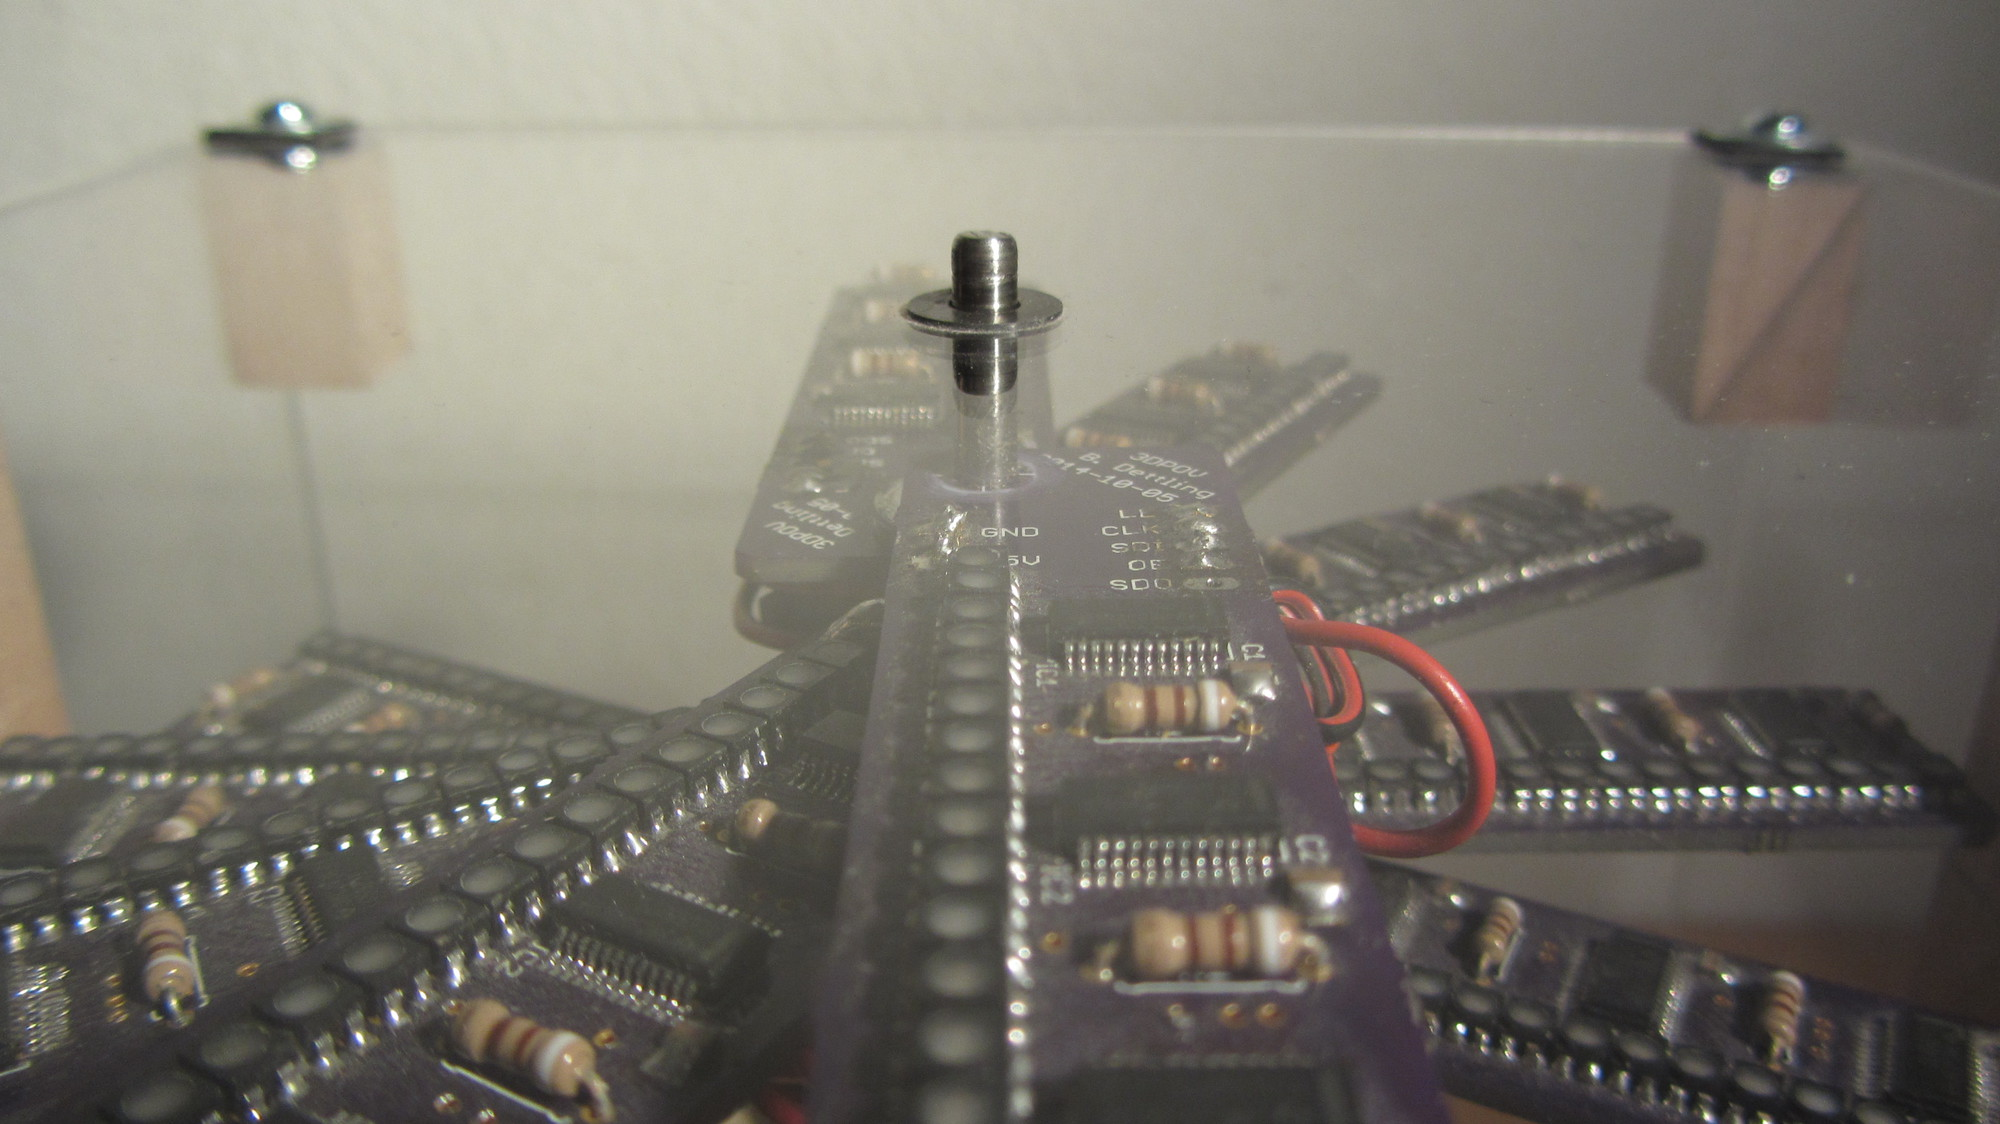
\includegraphics[width=0.9\paperwidth]{./images/cover.jpg}}

    \vspace*{1cm}
    \Large
    Balduin Dettling

    \large
    Matura Project 2014 \\ Kantonsschule Wiedikon

    Mentored by Patrick Spengler and Prof. Heinz Domeisen
    \vfill

\end{titlepage}


\section{Introduction}

\pagenumbering{arabic}

3D Displays are becoming increasingly common: Movies can be viewed in 3D cinemas, and people even
have 3D television screens in their living room. However, these displays don't actually display
depth, they merely provide an illusion of it. They work by projecting images from slightly
different viewpoints to each eye, letting the human brain figure out depth information.

In this work, however, I built a display that is actually three-dimensional. It can be viewed from
any direction, and pixels are distributed across three spatial dimensions. Such a display is
called a persistence of vision display or a swept-volume display. It uses a rapidly rotating
two-dimensional arrangement of LEDs. By controlling it precisely, it can display a still
three-dimensional image.

The idea to build such a display came from two-dimensional displays building upon the same
principle; building them is quite a popular project among tinkerers and engineers alike. I
initially had in mind to make another 2D display, but since there are instruction manuals online I
didn't see much of a point in doing so. Instead I went one step further and built a
three-dimensional version.

In my display, 160 pixels are distributed across ten circuit boards. All LEDs are controlled by a
Teensy 3.1 microcontroller and 30 LED drivers. They are refreshed 100 times per rotation, for a
total of 16000 voxels. The display rotates at about \SI{60}{\hertz}, which is enough for the image
to not flicker. By measuring the rotational speed with a hall effect sensor, the image stays in
place despite the rotational speed not being exactly constant.

A python program facilitates the creation of images: It can insert straight lines, spheres,
cuboids, planes and even plots of arbitrary functions into the an image, which can then be loaded
onto the Teensy and shown on the 3D display.


\section{Hardware}

\subsection{Components}

\subsubsection{Control}

For controlling the LEDs, I used a Teensy 3.1 microcontroller development board. Its small
footprint is ideal for the fast rotation. With a clock speed \SI{96}{\mega\hertz} and a register
width of \SI{32}{\bit}, it's powerful enough to rapidly control a large amount of LEDs.

The controller has to have some kind of reference point, so that it can calculate the current
speed and angular position of the device. For this, I used a hall effect sensor on the rotating
side, which passes by a stationary magnet after each rotation.

This microcontroller can't control all 480 LEDs on its own, which is why I used LED drivers.
Specifically, I used the TLC5927 by Texas Instruments. These chips essentially consist of a
\SI{16}{\bit} shift register with some extra features, the most important of them being constant
current regulation.


\subsubsection{LEDs}

The LEDs I used are surface-mounted RGB leds with a diffused lens and a width of
\SI{2.8}{\milli\meter}. Their small size makes them ideal to use as pixels, and the diffused lens
causes the colors mix well, even when viewed directly.

\subsubsection{Motor}

In order to make the whole device rotate, I salvaged a brushed DC motor from an old RC motor boat.
Because of its high torque, I could attach the motor directly to the rotating shaft instead of
using gears or a belt drive. That way there are less moving parts and the motor can turn at a
lower rotational speed, both resulting in less wear and noise.


\subsubsection{Power Transmission}

Power is transmitted from the stationary power supply to the rotating electronics by a pair of
slip rings. I made them out of two round pieces of copper sheet on the rotating end, and two long
pieces of copper sheet on the stationary part.

In order to supply 480 LEDs with \SI{20}{\milli\ampere} each, a current of \SI{9.6}{\ampere} is
necessary. Testing has shown that the slip rings don't cause a significant voltage drop at this
current. In practice, however, the average current is much lower since most pixels are switched
off in a typical 3D image.

Because two pieces of copper rubbing against each other aren't the most reliable electrical
connection, I used a \SI{2200}{\micro\farad} electrolytic capacitor to smooth out the supply
voltage.


\subsection{Circuit Diagram}

\begin{figure}[h]
\vspace{0mm}
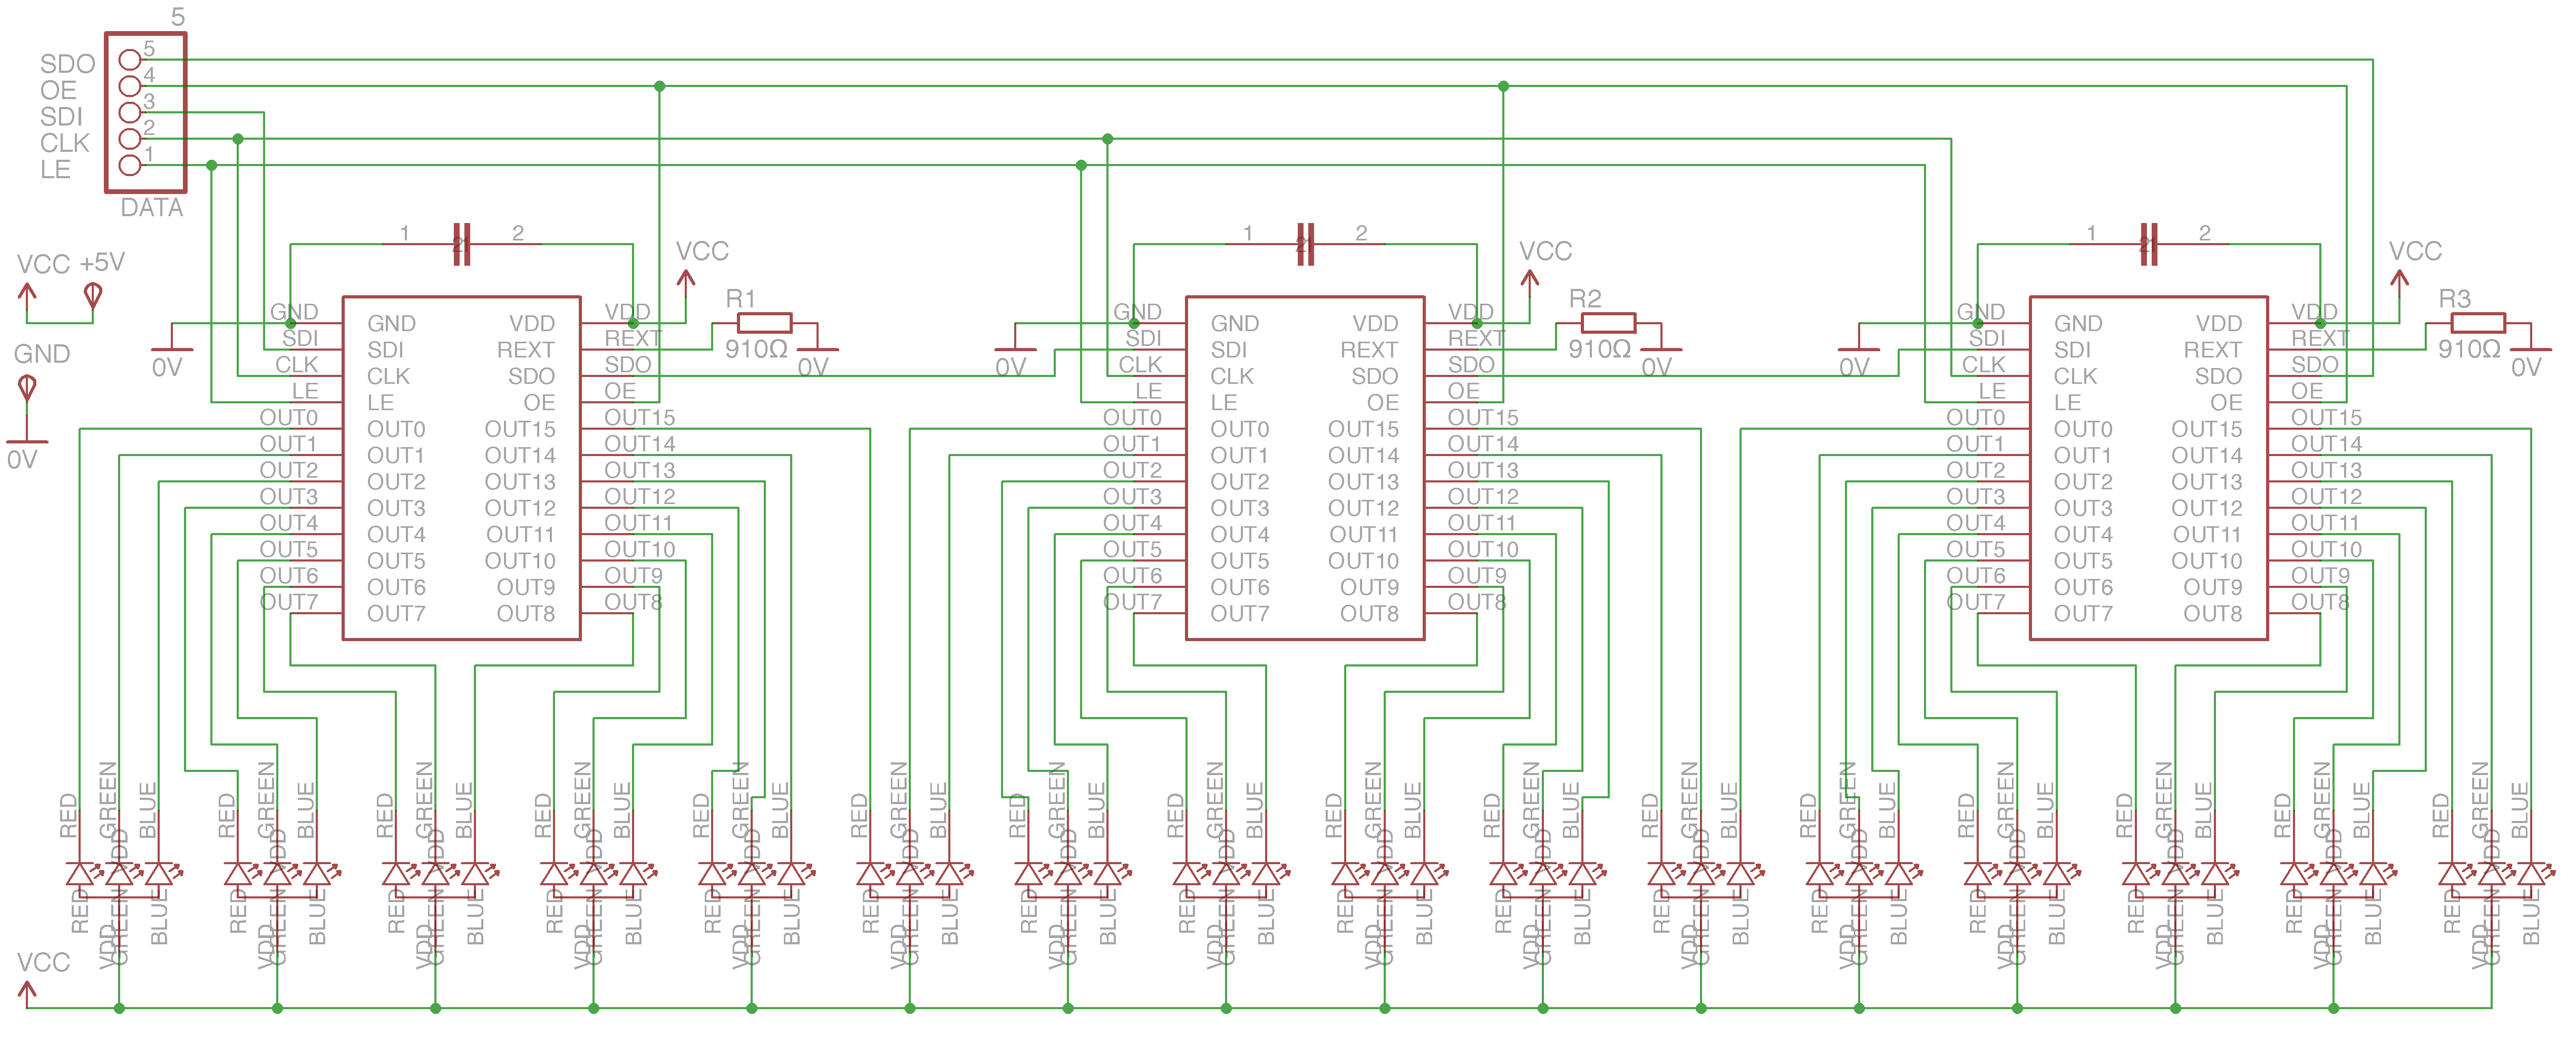
\includegraphics[width=\textwidth]{./images/schematic.png}
\vspace{-10mm}
\caption{The finished circuit diagram}
\vspace{4mm}
\end{figure}

The circuit diagram --- as well as the PCB layout --- were created in Eagle. Its free version is
limited to two-layer boards of sizes up to \SI{10}{\centi\meter} by \SI{8}{\centi\meter}, but
that's more than enough for my purposes.

The LED drivers are arranged in a daisy chain configuration, where the serial data output of each
chip is connected to the serial data input of the next chip. This is not only the case within one
board, but also between the different boards: The data output of one board is connected to the
next board's input. That way, all 30 LED drivers can be controlled by a single SPI bus.

\def \iout {I\textsubscript{OUT}\xspace}
\def \rext {R\textsubscript{EXT}\xspace}

The external resistor connected to each LED driver sets the output current. The following
equation, taken from page 15 in the datasheet, describes the relation between the output current
(\iout) and the resistor's value (\rext):

% Lots of ugly hacks to have a non-italic font
\begin{ownmath}
\textrm{\iout} = 15 \cdot \frac{\SI{1.25}{\volt}}{\si{\rext}}
\end{ownmath}

% \frac{\SI{1.25}{\volt}}{\SI{\rext}}
For an output current of \SI{20}{\milli\ampere}, \rext needs to be \SI{937.5}{\ohm}. The next
smaller value within the E24 series is \SI{910}{\ohm}, which is what I ultimately used.

A \SI{1}{\micro\farad} bypass capacitor is located close to each LED driver so that their power
consumption can change almost instantly without causing a spike in the supply voltage.

I used a row of 5 pins to transmit data to the LED drivers. The data lines (serial data in
and out) are connected to the input of the first chip and the output of the last chip
respectively. The rest of the pins (clock, output enable and latch enable) are control lines,
which go to all three chips simultaneously.

\subsection{PCB Design}

The above schematic translates directly to the PCB layout, which was also created in Eagle. The
most important consideration was to save as much space as possible, which I did simply by placing
parts as close as possible to each other. The supply lines are routed on top of each other so
their magnetic fields (which can change quickly) are largely cancelled out.

\begin{figure}[h]
\vspace{4mm}
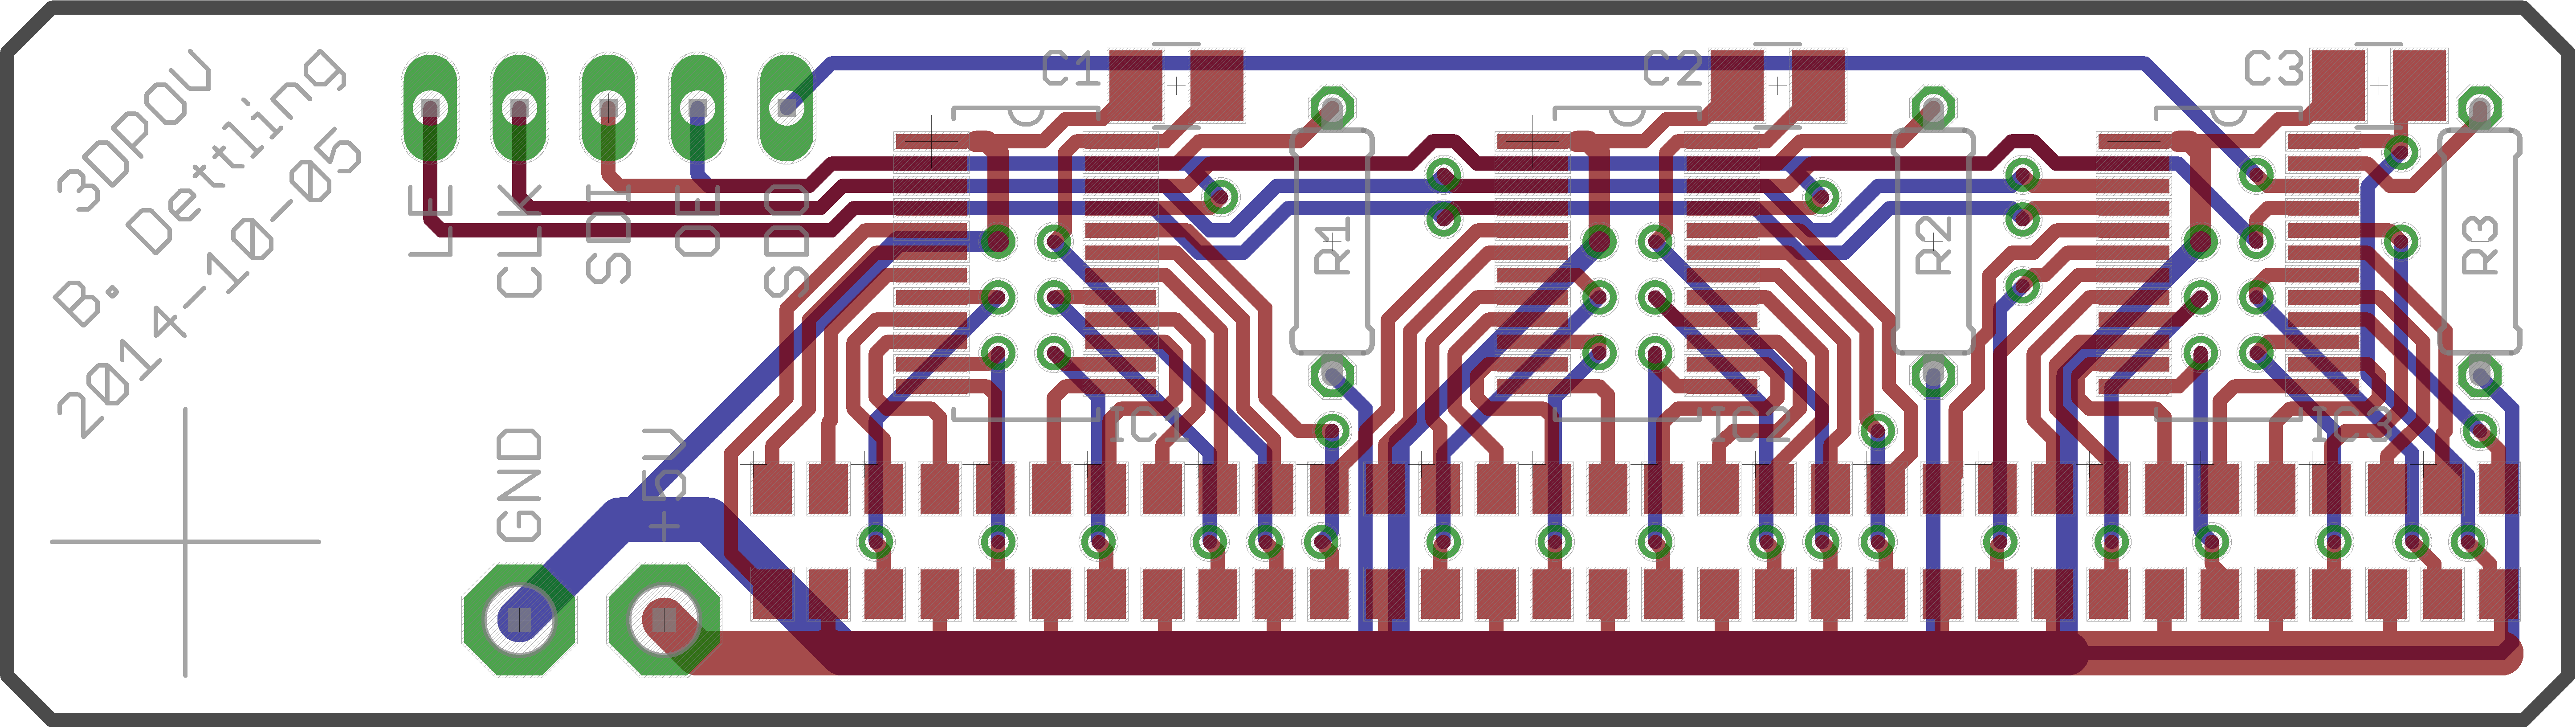
\includegraphics[width=\textwidth]{./images/board-layout.png}
\vspace{-8mm}
\caption{The PCB layout in Eagle.}
\vspace{-5mm}
\end{figure}


\section{Fabrication}

\subsection{Circuit Boards}

I ordered 12 PCBs with the above layout at \url{https://oshpark.com/}, which has cost me 47 USD.
20 days later, the finished boards arrived at my doorstep.

\begin{figure}[h]
\vspace{3mm}
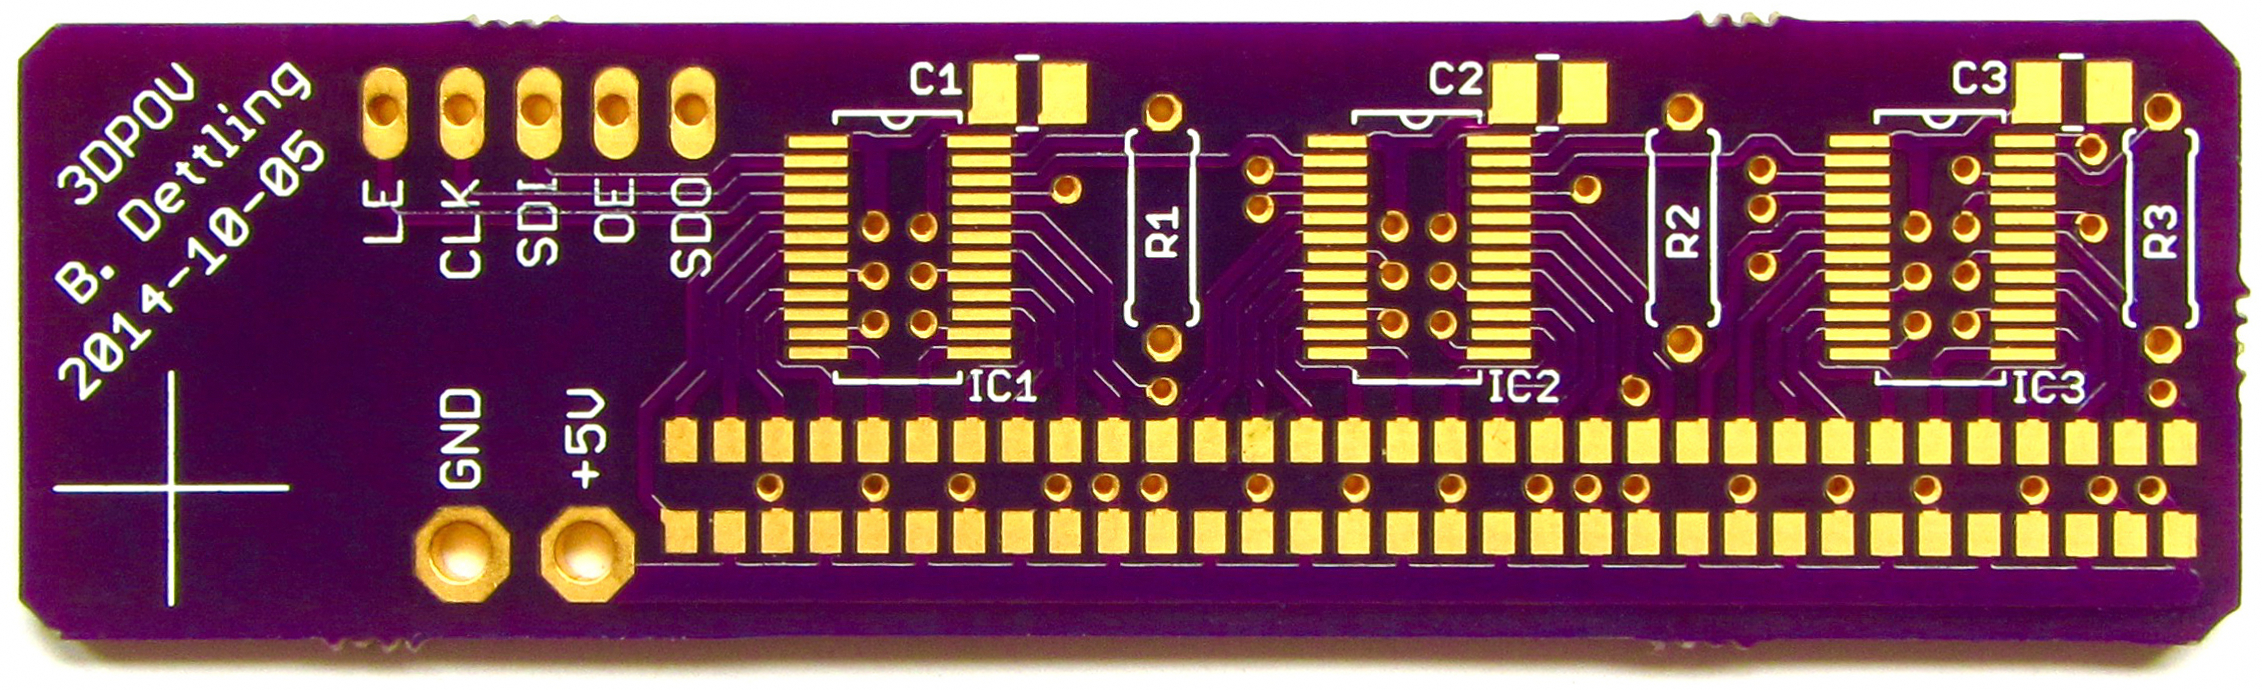
\includegraphics[width=\textwidth]{./images/board-finished.jpeg}
\vspace{-10mm}
\caption{A finished circuit board}
\vspace{2mm}
\end{figure}

Soldering the tiny, surface-mount LEDs to the board took some practice, but otherwise I
encountered no problems while equipping the boards with components.


\subsection{Physical Assembly}

The frame is built out of beech wood strips on a plywood plate. A horizontal board hosts the
motor, which in turn supports the rotating shaft with all the electronic on it.

Around the frame, I constructed an enclosure out of acrylic glass to protect the display and to
remove the risk of accidentally reaching into the rotating circuit boards.

The slip rings used to transmit power to the rotating electronics consist of two round pieces of
copper sheet on the rotating part, and two long pieces of copper sheet on the stationary part.
Unfortunately, they need a considerable amount of pressure to form a good enough contact, which
leads to quick wear as well as wasted electricity.

The microcontroller is mounted on another wooden disc, located a few centimetres above the slip
rings. The \SI{2200}{\micro\farad} capacitor as well as the hall sensor are also located on this
disc. The corresponding magnet is mounted on a piece of threaded rod, which itself is mounted on
the same board as the motor.

In the end, this place has become a bit of a mess, especially with all the cables going up to the
circuit boards. Luckily this isn't visible while the device is running.

Finally, I mounted the circuit boards on the shaft connected to the motor. There were two
important factors I had to consider while arranging the boards:

\begin{itemize}
\item The boards had to be balanced out to minimise static and dynamic unbalance
\item The amount of pixels obstructed by other circuit boards had to be minimal
\end{itemize}

I fulfilled both of these requirements by arranging the ten boards in a double-spiral arrangement.
This was the only arrangement I could think of that (theoretically) has no static imbalance at all
and minimal dynamic imbalance. On the viewer-facing half of the display, all LEDs are constantly
visible. On the backside, however, it's possible that one group of boards is right before the
other one, causing some layers of the image to disappear. When viewing the display from above,
almost all pixels except some of the innermost ones are visible.


\section{Programming}

\subsection{Timing}

In order to display a stable image, the program has to compensate for slight changes in rotational
speed. The hall effect sensor is used to measure the duration of one revolution. After this
measurement is made, the value is divided by 100 and stored in the variable
\texttt{microsPerPixel}, where it's interpreted as a reference for how long each pixel should be
displayed.

A variable called \texttt{nextPixelMicros} stores the time when the next pixel should be
displayed. As soon as this time has arrived, the function \texttt{sendData} is called and
\texttt{nextPixelMicros} is incremented by \texttt{microsPerPixel}, causing the program to wait
until the next pixel should be dispayed.


\subsection{Data storage and display}

The image is saved in a three-dimensional array of $100 \cdot 10 \cdot 6$ bytes. The first index
stands for the angle of a pixel in hundredths of a circle, the second index for the height and the
third one for the position of each byte on a row of LEDs. Because there are 48 LEDs per row, 6
bytes can be used to describe the row's state without wasting any storage space.

The previously mentioned function \texttt{sendData} needs to be able to know which bytes to send
based on the current angle of of the display. Because the PCBs are not right above each other, the
bytes that are being sent out at the same time don't correspond to the pixels that are above each
other in the image. The program accounts for these offsets by calculating the position of each
board relative to the first one and sending the according values out of the saved image.


\subsection{Image Creation}

Initially, I created all the 3D images by hand, which was a tedious and error prone task. In order
to simplify it, I wrote a python program that would support me in making images. All of the source
code is available on \url{https://github.com/mbjd/\_3DPOV} in the folder \texttt{image\_creation}.

In order to save an image in this program, I used a three-dimensional array of $100 \cdot 10 \cdot
16$ integers.  The lowest three bits of each integer represent the states of the red, green and
blue LED respectively. In comparison to the data format used on the display itself, this takes up
more memory but is much simpler to edit.

The program can create simple shapes such as straight lines, planes, spheres, cuboids or arbitrary
polygons. It can also plot any given function of the signature $f(x,y) \mapsto z$, $f(x,y,z)
\mapsto \text{colour}$, or $f(x,y,z) \mapsto \{0, 1\} $, where x, y, and z are the three axes of
the cartesian coordinate system.

Once an image is complete, it can be converted to a program for the Teensy 3.1 with a single
function call.


\section{Conclusions}

\subsection{Possible Improvements}

The display works as initially planned and can display volumetric images with a resolution of $16
\cdot 10 \cdot 100$ pixels and a colour depth of \SI{3}{\bit}. It's also something that most
people have never seen, which makes them interested in the display. However, there are several
aspects that could be improved upon.

\subsubsection{Slip Rings}

Because the slip rings are quite rough, substantial pressure is needed to form a consistent
contact. This leads to a lot of friction and quick wear of the contacts.

This problem could be solved by replacing the slip rings with two coils for inductive power
transfer. While this would be a more complicated solution, it would significantly reduce friction
and noise while transmitting power more reliably.


\subsubsection{Image creation}

The program I wrote facilitates creating simple images with geometric shapes. However, the only
way to make more complicated images is to set each pixel by hand. A more flexible solution would
be a program that takes a 3D model in a widely used file format and converts it to be displayable
on my display, so users can create their images in any 3D graphics program.


\subsubsection{Memory Space}

Since the Teensy 3.1 only has \SI{256}{\kilo\byte} of flash memory, the amount of images that can
be stored is very limited. For static images this is fine, but animations can have a length of
only 42 frames before running out of space.

In order to get around this limit, external storage would be necessary, for example in the form of
an SD card. Even with \SI{1}{\giga\byte}, I could save 166666 frames, thus removing any practical
limit in terms of playback time.


\subsubsection{Interactive Programs}

It would be interesting to not only display predefined images, but to actually run a program that
can respond to user input. In order to communicate with the external world, a wireless interface
would be necessary. Readily available solutions include small WLAN or bluetooth modules, or the
transmitters and receivers commonly used in radio-controlled aircraft.

\subsection{Applications}

Because of the low resolution and colour depth, the high level of noise, quick wear and the
inability to send images to the display while running, this display is not suited as a replacement
for a computer or TV screen. However, these problems can all be fixed completely or partially, so
that there could one day exist a version of my display which is actually suitable for the above
purposes.

One domain where I could imagine a display like mine being especially useful is advertising.
Because most people haven't ever seen such a display before, it would be an immediate eye-catcher
in the display window of any business.

Furthermore, a display like mine would certainly be useful in educational settings. By visualising
things like atomic orbitals, the earth's structure, orbital mechanics or meteorologic phenomena on
a 3D display rather than on paper, these topics could be understood more easily.

Another fun thing to try would be video games. Although the limited resolution and computing power
would make it difficult to run the latest and greatest games, 3D versions of classics like Pong,
Snake or a simple platform game would certainly be worth a shot.

\end{document}

